\documentclass[a4paper,12pt]{report} % добавить leqno в [] для нумерации слева

%%% Работа с русским языком
\usepackage{cmap}					% поиск в PDF
\usepackage{mathtext} 				% русские буквы в формулах
\usepackage[T2A]{fontenc}			% кодировка
\usepackage[utf8]{inputenc}			% кодировка исходного текста
\usepackage[english,russian]{babel}	% локализация и переносы

\usepackage{graphicx}				%вставка изображений(графиков, в частности)
\usepackage{listings}
\usepackage{color}

\definecolor{dkgreen}{rgb}{0,0.6,0}
\definecolor{gray}{rgb}{0.5,0.5,0.5}
\definecolor{mauve}{rgb}{0.58,0,0.82}

\lstset{frame=tb,
  language=Python,
  aboveskip=3mm,
  belowskip=3mm,
  showstringspaces=false,
  columns=flexible,
  basicstyle={\small\ttfamily},
  numbers=none,
  numberstyle=\tiny\color{gray},
  keywordstyle=\color{blue},
  commentstyle=\color{dkgreen},
  stringstyle=\color{mauve},
  breaklines=true,
  breakatwhitespace=true,
  tabsize=4
}

%%% Дополнительная работа с математикой
\usepackage{amsmath,amsfonts,amssymb,amsthm,mathtools} % AMS
\usepackage{icomma} % "Умная" запятая: $0,2$ --- число, $0, 2$ --- перечисление

%% Номера формул
\mathtoolsset{showonlyrefs=true} % Показывать номера только у тех формул, на которые есть \eqref{} в тексте.

%% Шрифты
\usepackage{euscript}	 % Шрифт Евклид
\usepackage{mathrsfs} % Красивый матшрифт

%% Свои команды
\DeclareMathOperator{\sgn}{\mathop{sgn}}

\usepackage{parskip}
%\setlength\parindent{0ex}
%\setlength\parskip{0.3cm}

\renewcommand{\arraystretch}{1.8}

%%% Заголовок
\author{Волков Павел А-14-19}
\title{Отчет по Лабораторной работе №6}
\date{\today}

\begin{document}

\begin{titlepage}
	\newpage

	\begin{center}
	НАЦИОНАЛЬНЫЙ ИССЛЕДОВАТЕЛЬСКИЙ УНИВЕРСИТЕТ\\
		"МОСКОВСКИЙ ЭНЕРГЕТИЧЕСКИЙ ИНСТИТУТ"\\
	\end{center}

	\vspace{8em}	

	\begin{center}
		\Large Кафедра математического и компьютерного моделирования\\ 
	\end{center}

	\vspace{2em}

	\begin{center}
		\textsc{\textbf{ \Large Численные методы \linebreak Отчет по лабораторной работе №5 \linebreak "Численное интегрирование." \linebreak Вариант 52}}
	\end{center}

	\vspace{6em}



	\newbox{\lbox}
	\savebox{\lbox}{\hbox{Амосова Ольга Алексеевна}}
	\newlength{\maxl}
	\setlength{\maxl}{\wd\lbox}
	\hfill\parbox{11cm}{
		\hspace*{5cm}\hspace*{-5cm}Студент:\hfill\hbox to\maxl{Волков Павел Евгеньевич\hfill}\\
		\hspace*{5cm}\hspace*{-5cm}Преподаватель:\hfill\hbox to\maxl{Амосова Ольга Алексеевна}\\
		\\
		\hspace*{5cm}\hspace*{-5cm}Группа:\hfill\hbox to\maxl{А-14-19}\\
	}


	\vspace{\fill}

	\begin{center}
		Москва \\2021
	\end{center}

\end{titlepage}
\section*{Задача 6.1}
\subsection*{Постановка задачи}
Исследовать поведение погрешностей при численном дифференцировании функции.
\[
\begin{array}{| c | c | c |}
	\hline
	№ & f(x) & [a, b] \\ \hline
	5.2.52 & 6e^{-x}\sin{2\pi x} & [0, 3] \\ \hline
\end{array}
\]
\subsection*{Решение}
Для вычисления производной в точке $c = 0.9$ будем использовать 2 формулы - правой и левой разностной производной:
\begin{gather}
	f'(x) \approx \dfrac{f(c + h_k) - f(c)}{h_k}\\
	f'(x) \approx \dfrac{f(c) - f(c - h_k)}{h_k}
\end{gather}

Приведем графики погрешностей вычисления производных 1-го и 2-го порядка в точке $c = 0.9$.

\begin{figure}[h!]
	\centering                                                                                            
	\begin{minipage}{0.45\textwidth}
	        \centering
	        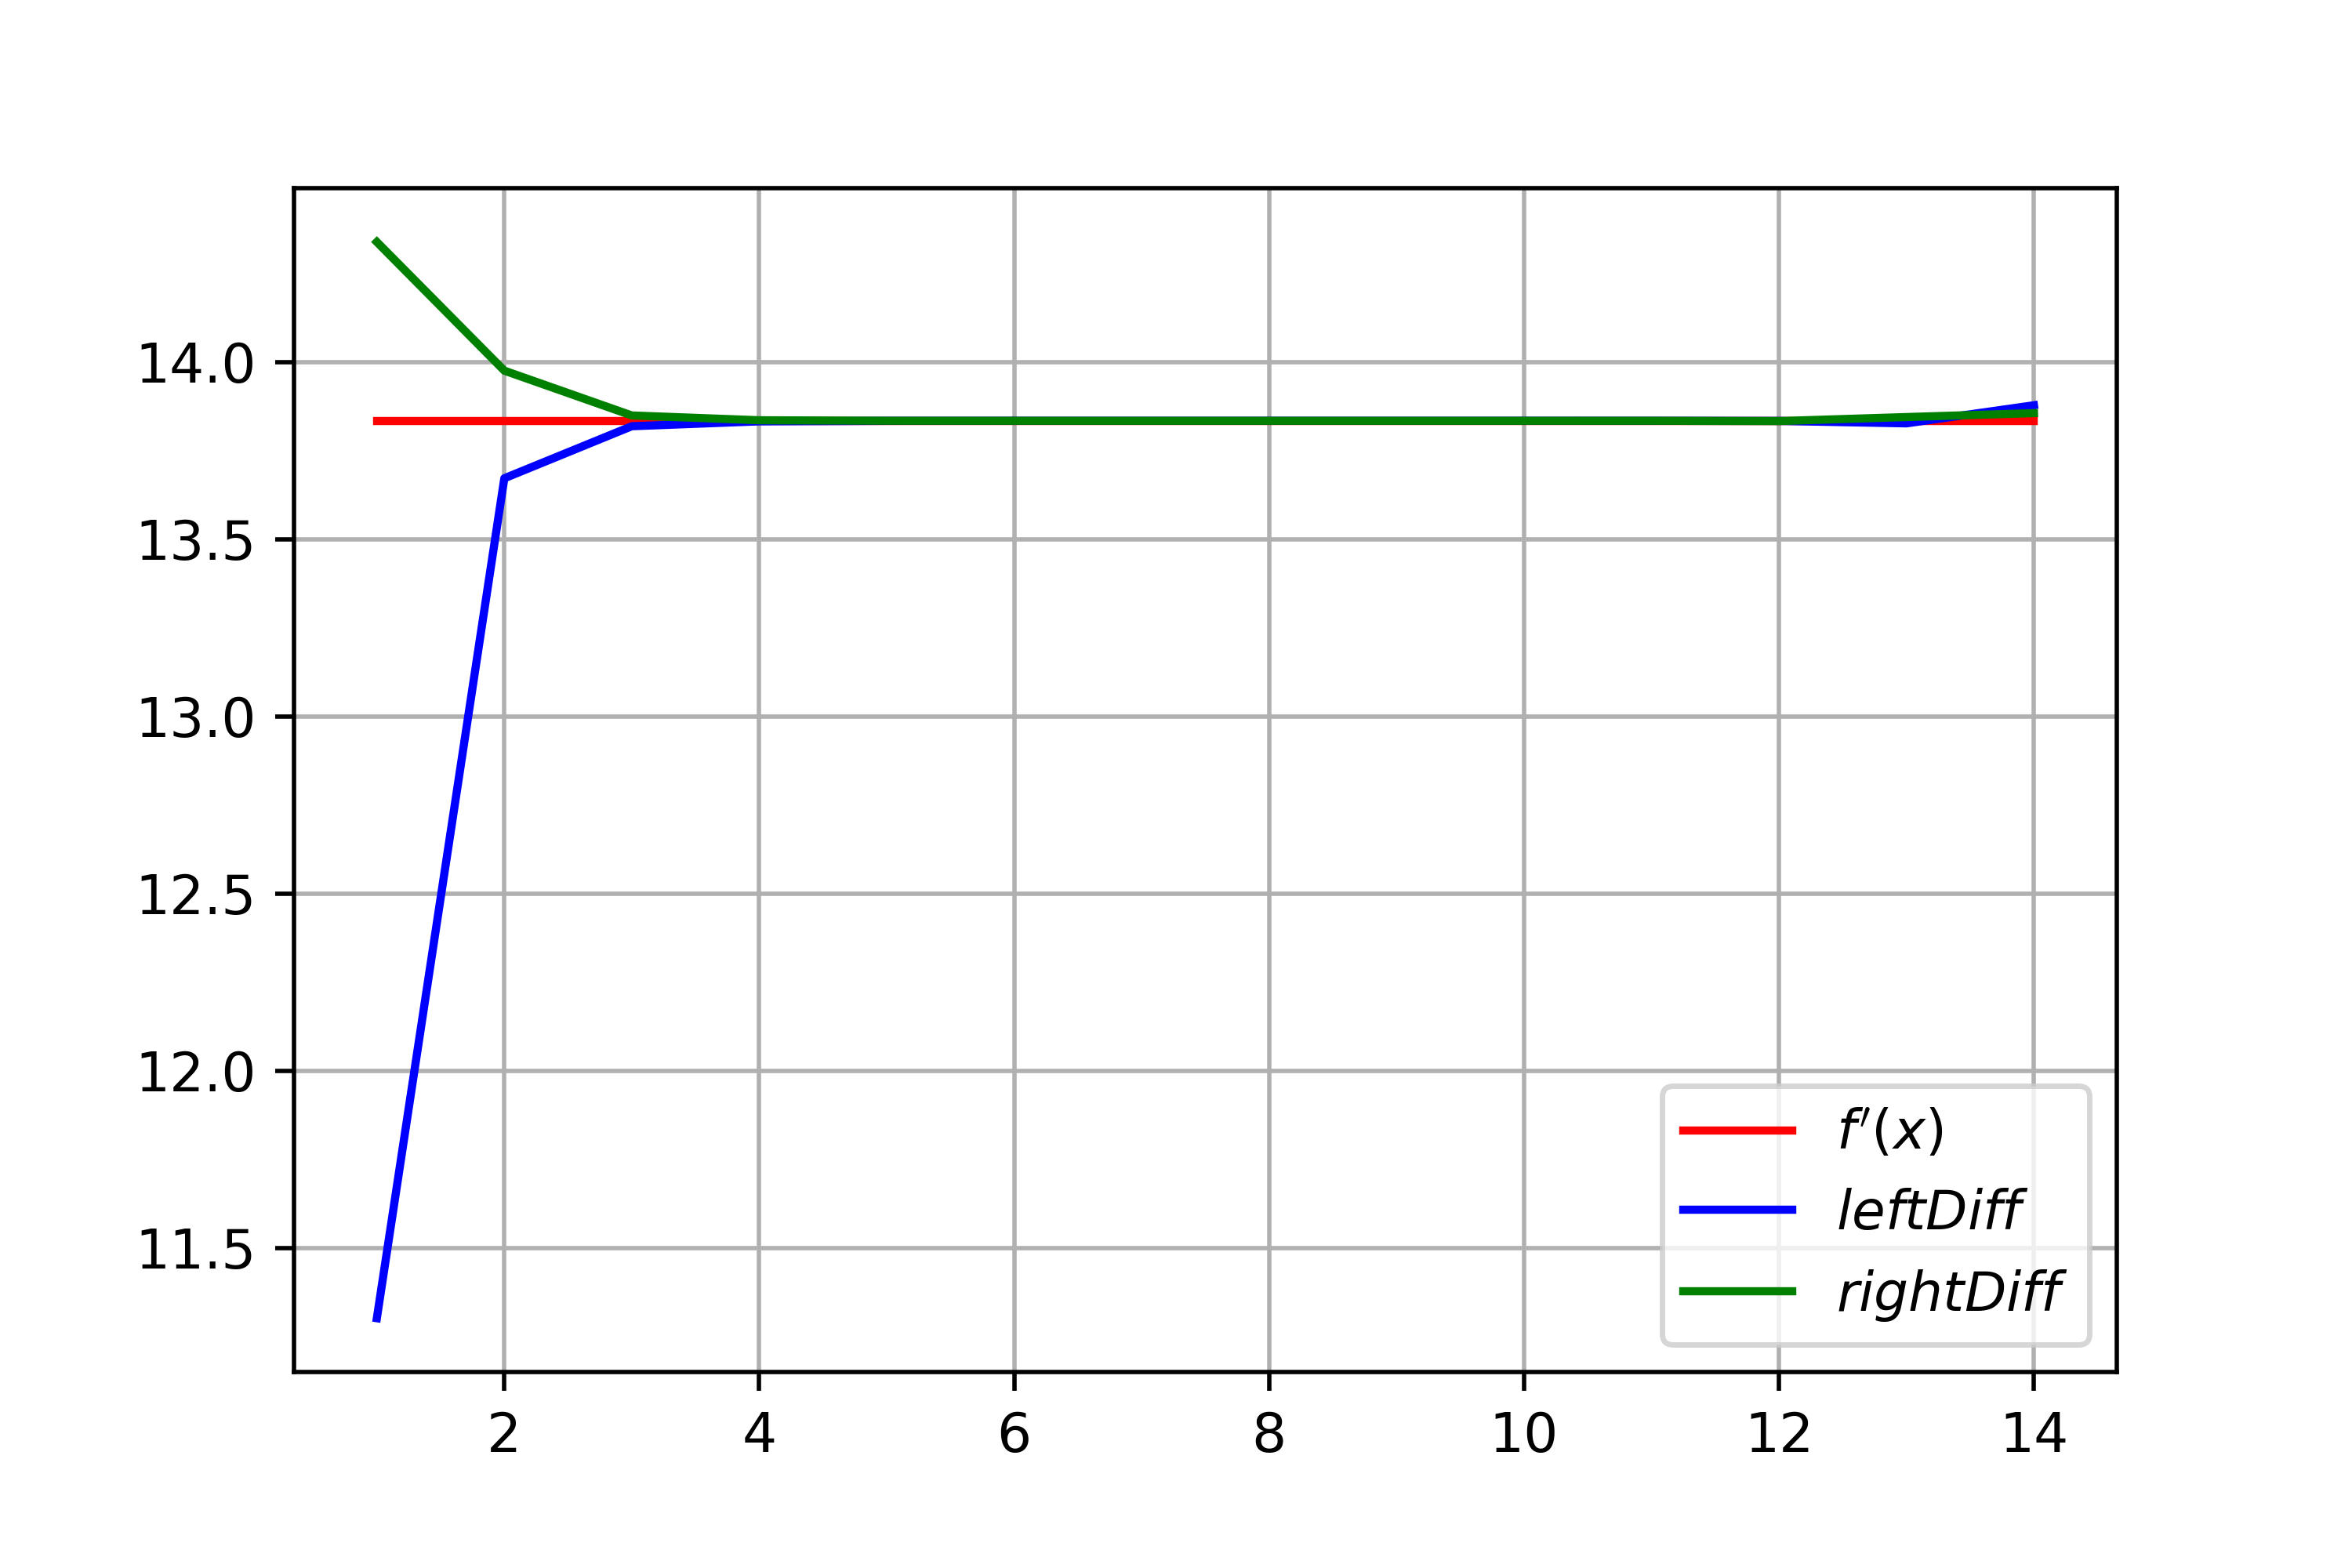
\includegraphics[width=8.5cm]{images/plot_6.1_1st_deriv.png} % первое изображение
	        \caption{Графики производных 1-го порядка, вычисленных с помощью формул левых и правых разностных производных}
	\end{minipage}\hfill
	\begin{minipage}{0.45\textwidth}
		\centering
		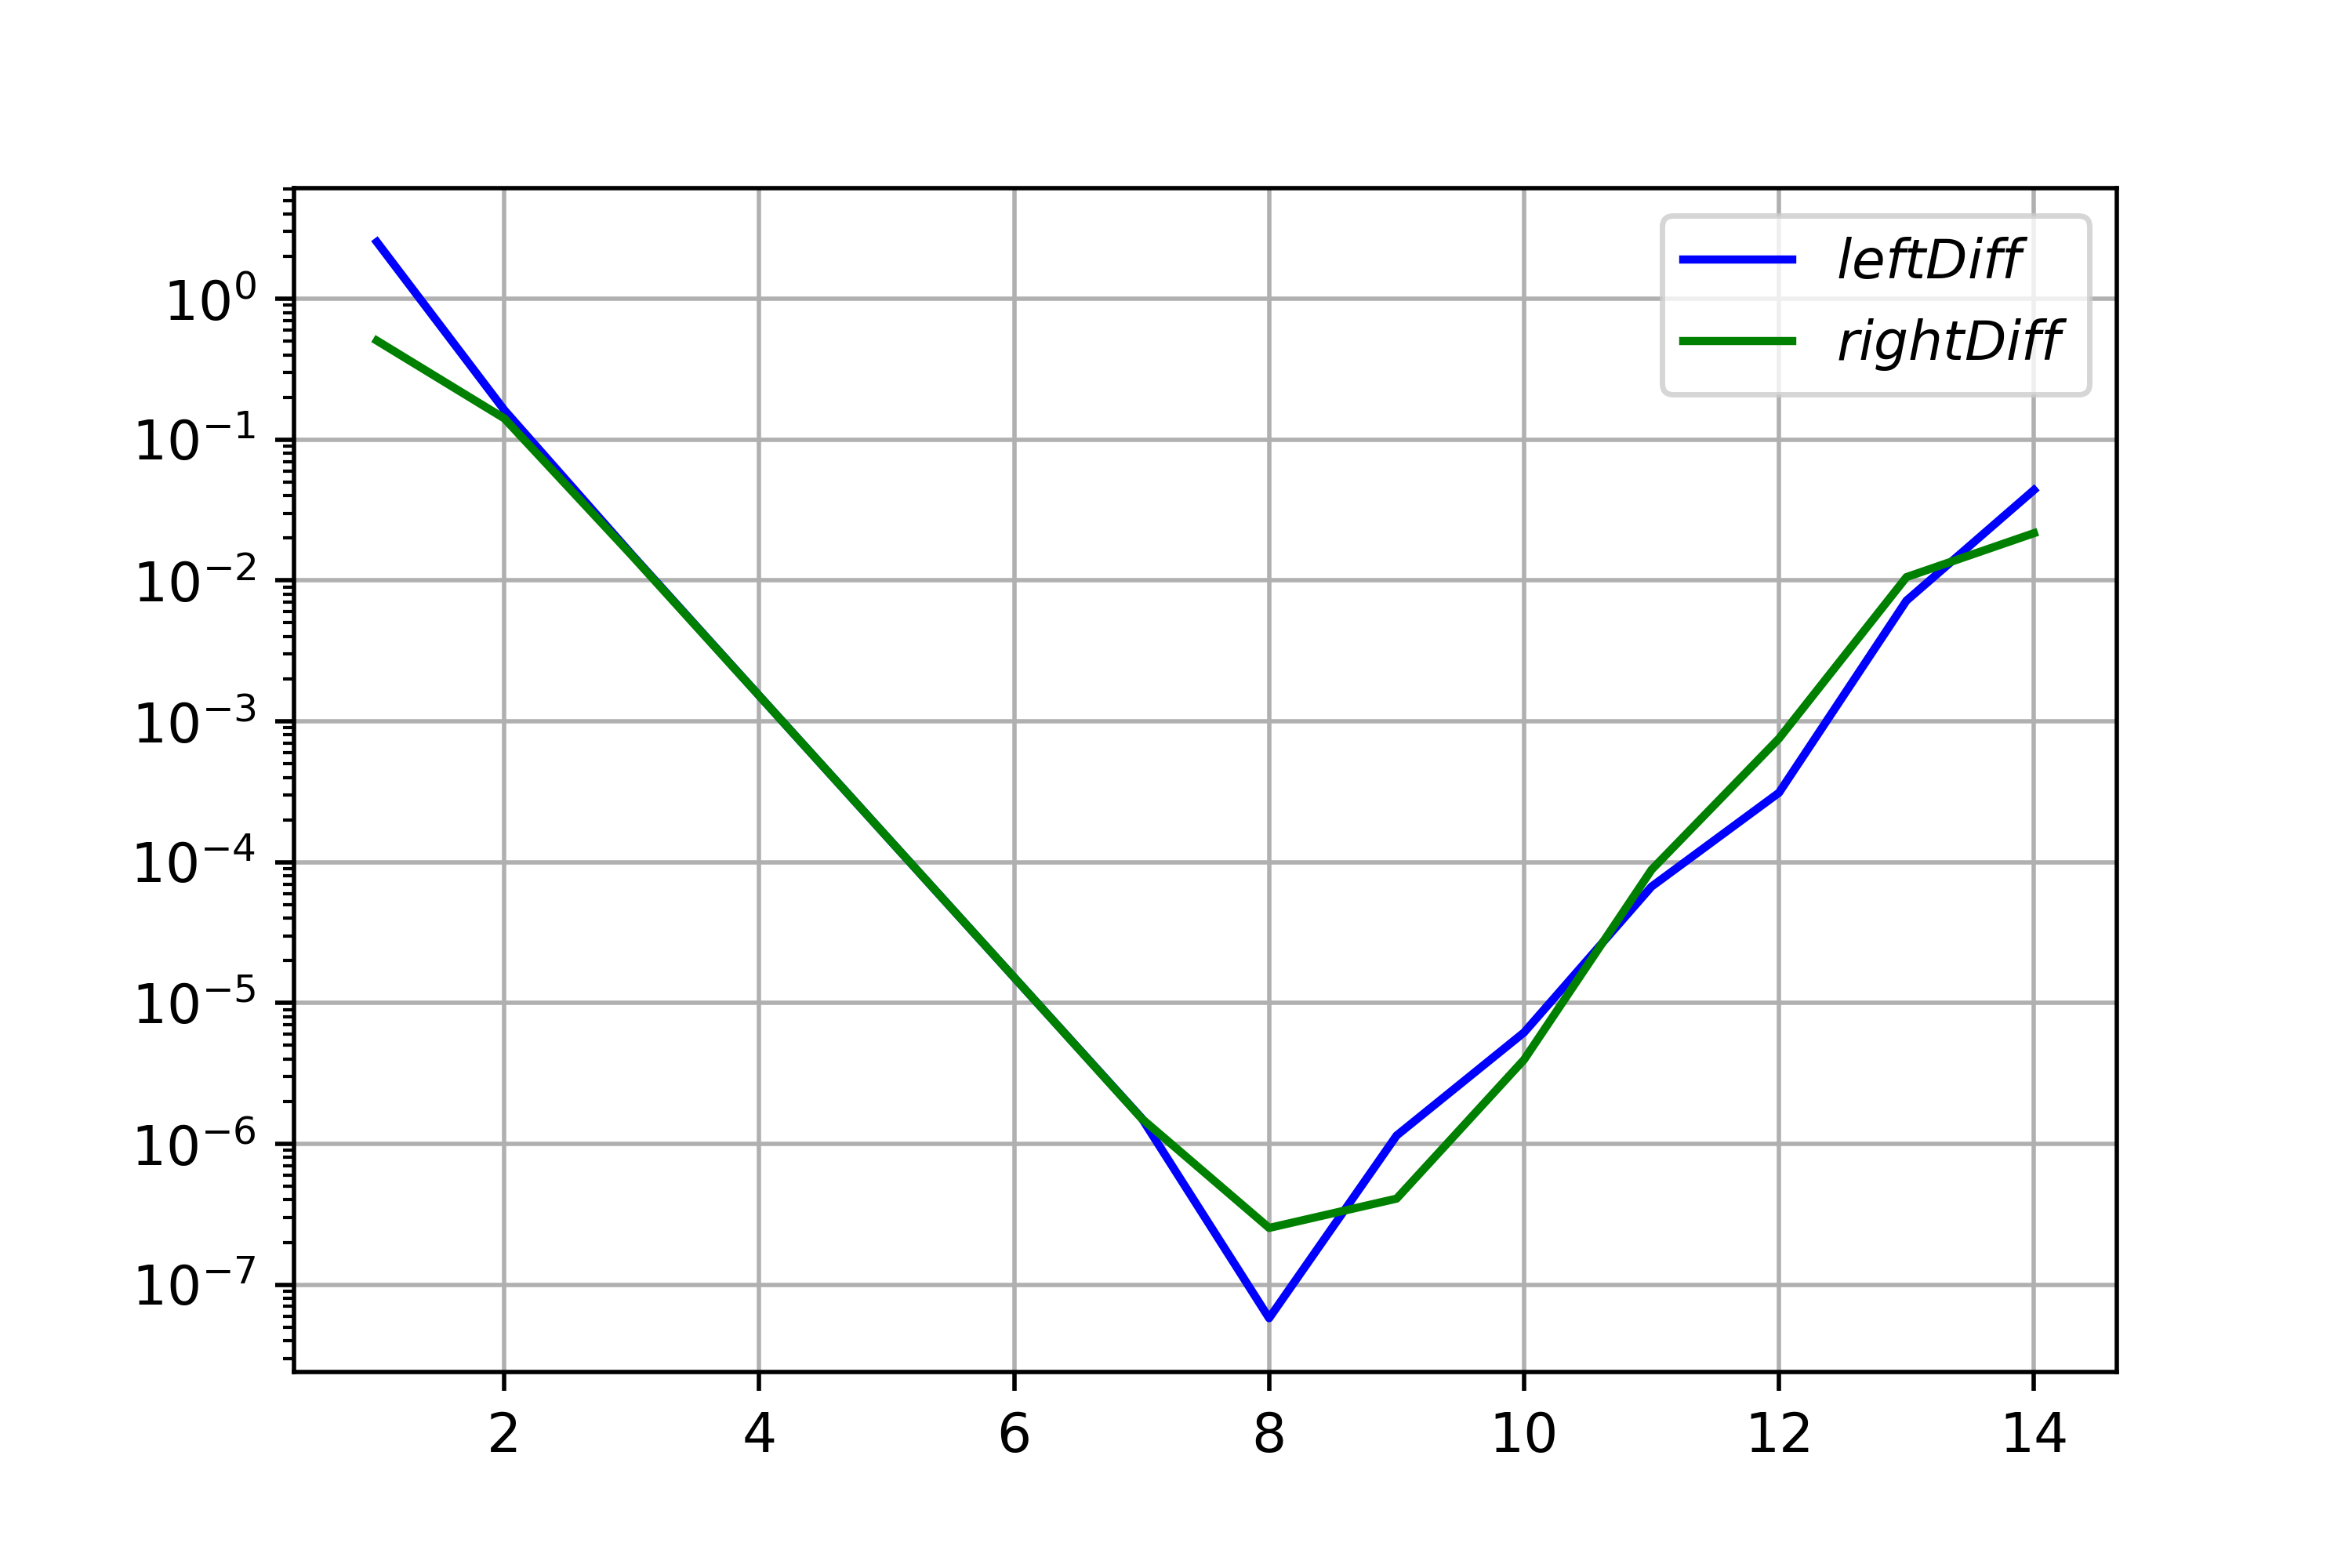
\includegraphics[width=8.5cm]{images/plot_6.1_1st_deriv_err.png} % второе изображение
		\caption{Графики погрешностей вычисления первой производной  по левой и правой формулам разностных производных}
	\end{minipage}
\end{figure}

\begin{figure}[h!]
	\centering                                                                                            
	\begin{minipage}{0.45\textwidth}
	        \centering
	        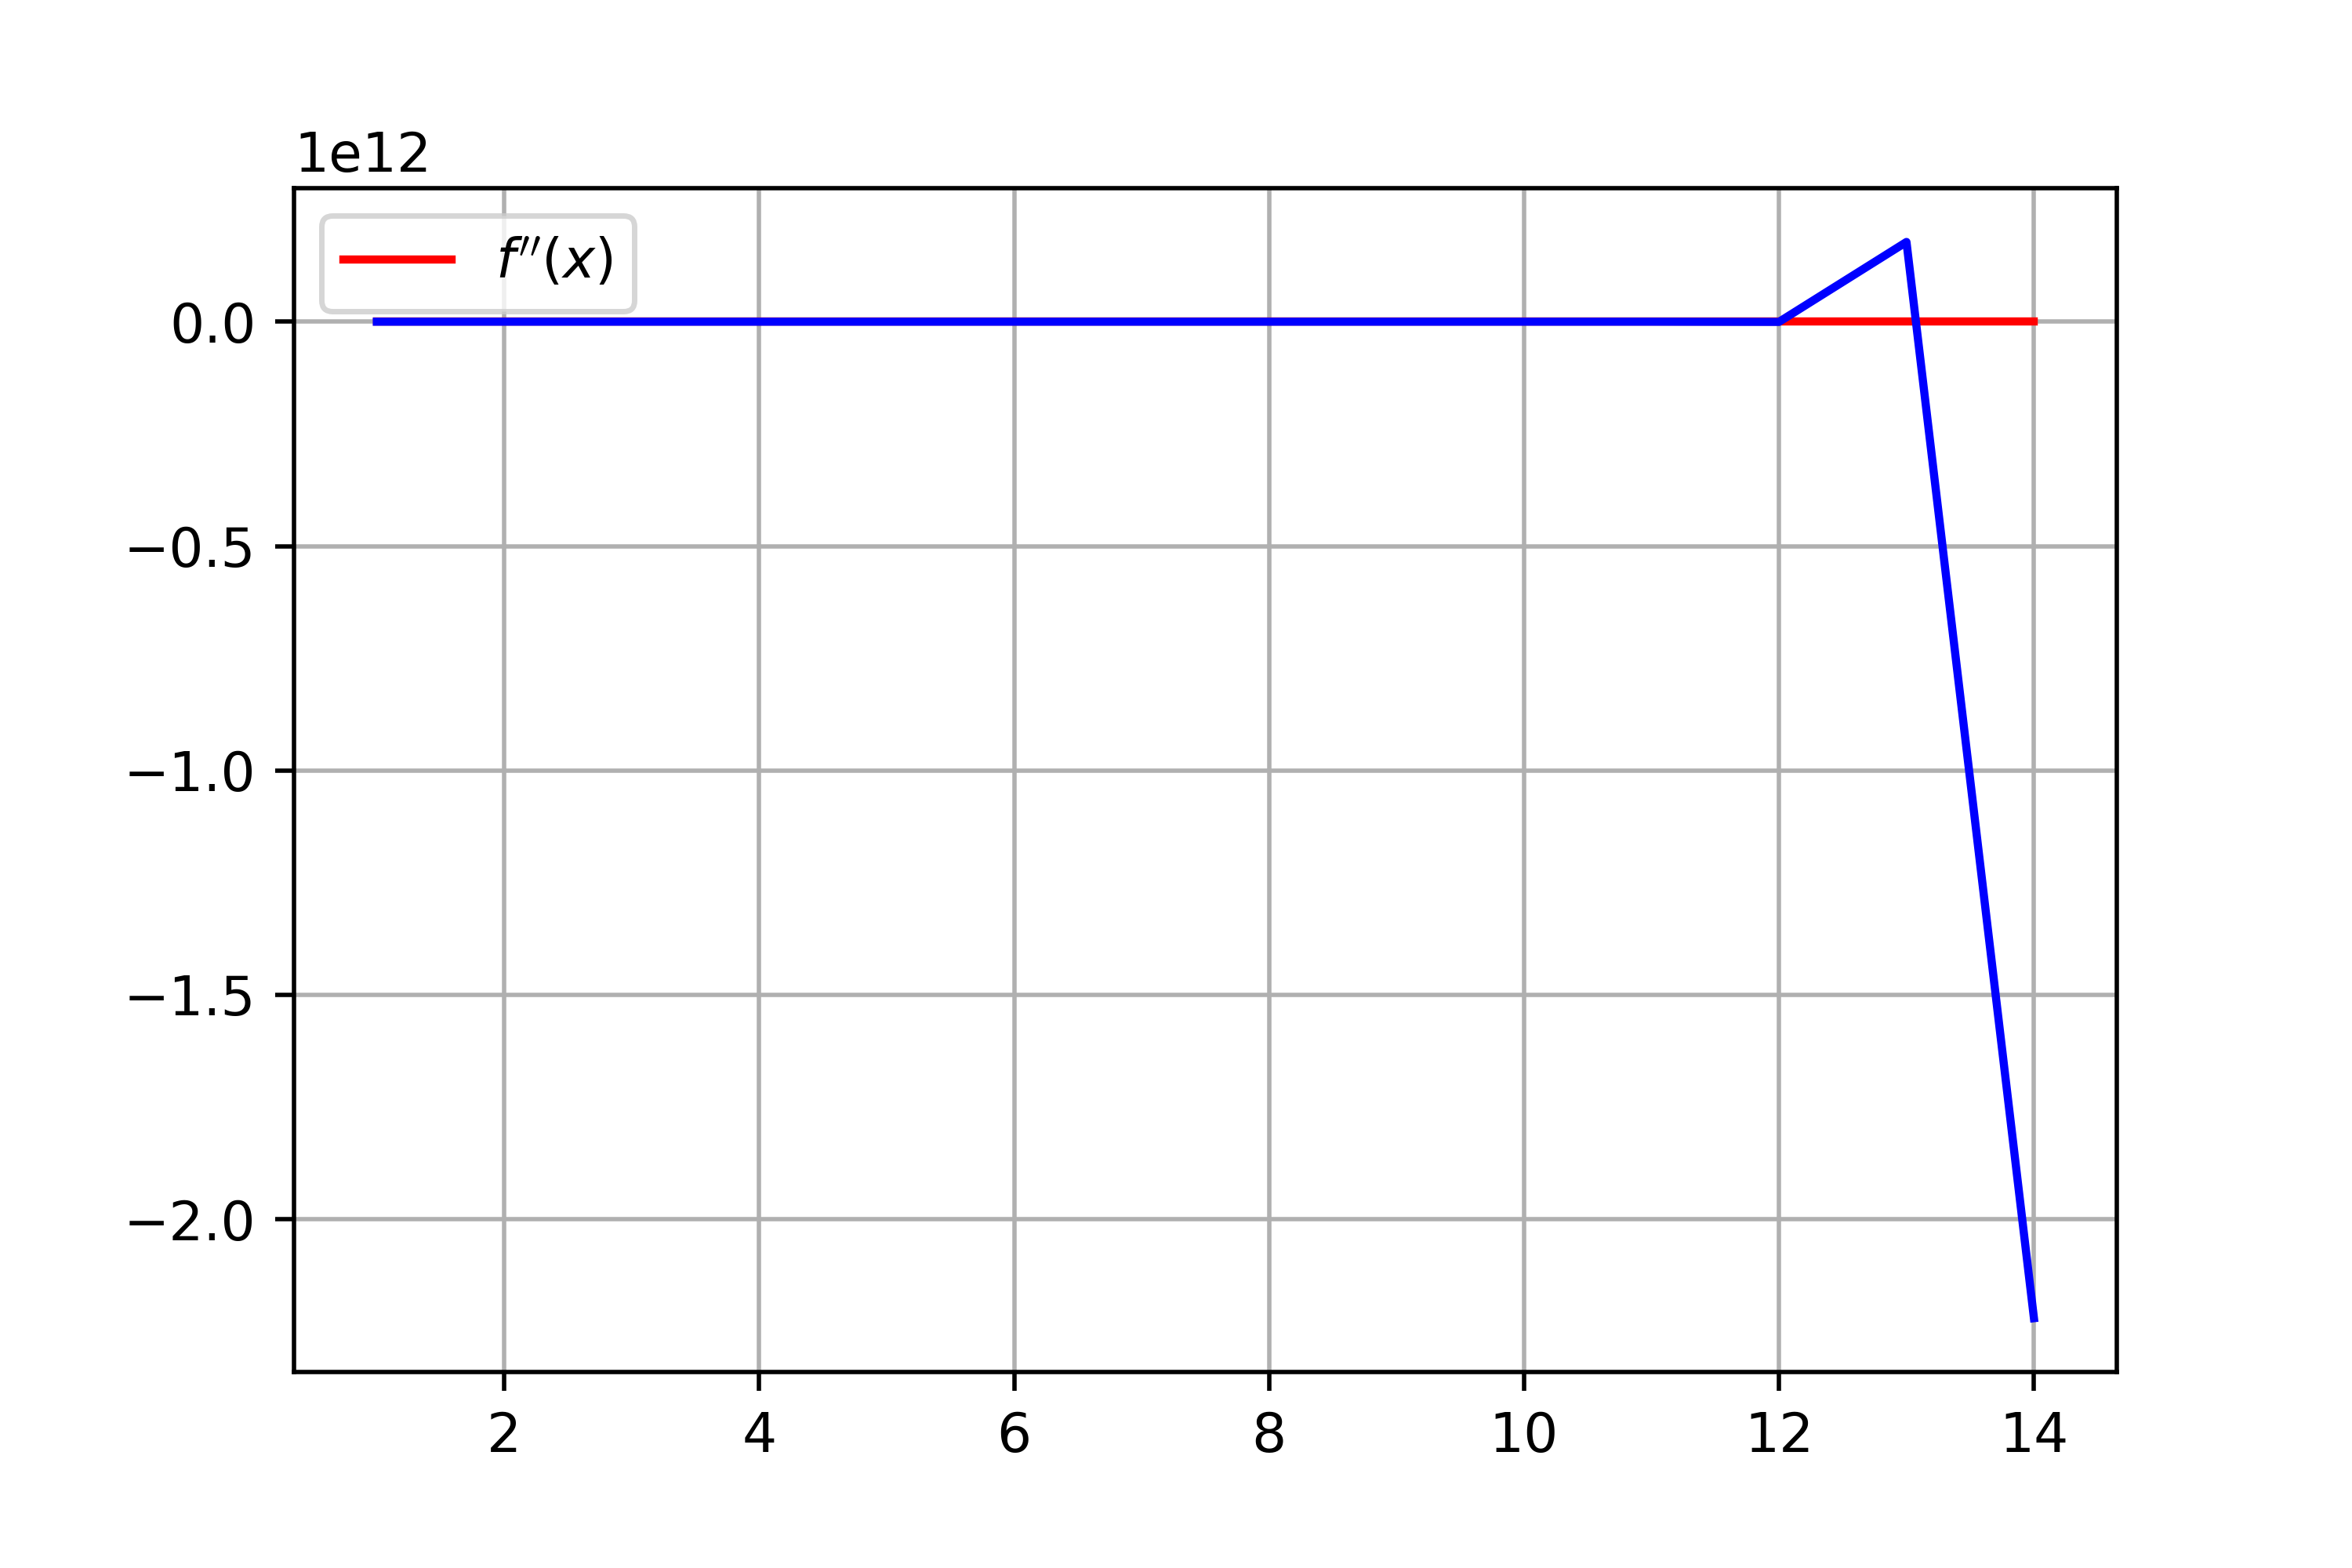
\includegraphics[width=8.5cm]{images/plot_6.1_2nd_deriv.png} % первое изображение
	        \caption{График производной 2-го порядка}
	\end{minipage}\hfill
	\begin{minipage}{0.45\textwidth}
		\centering
		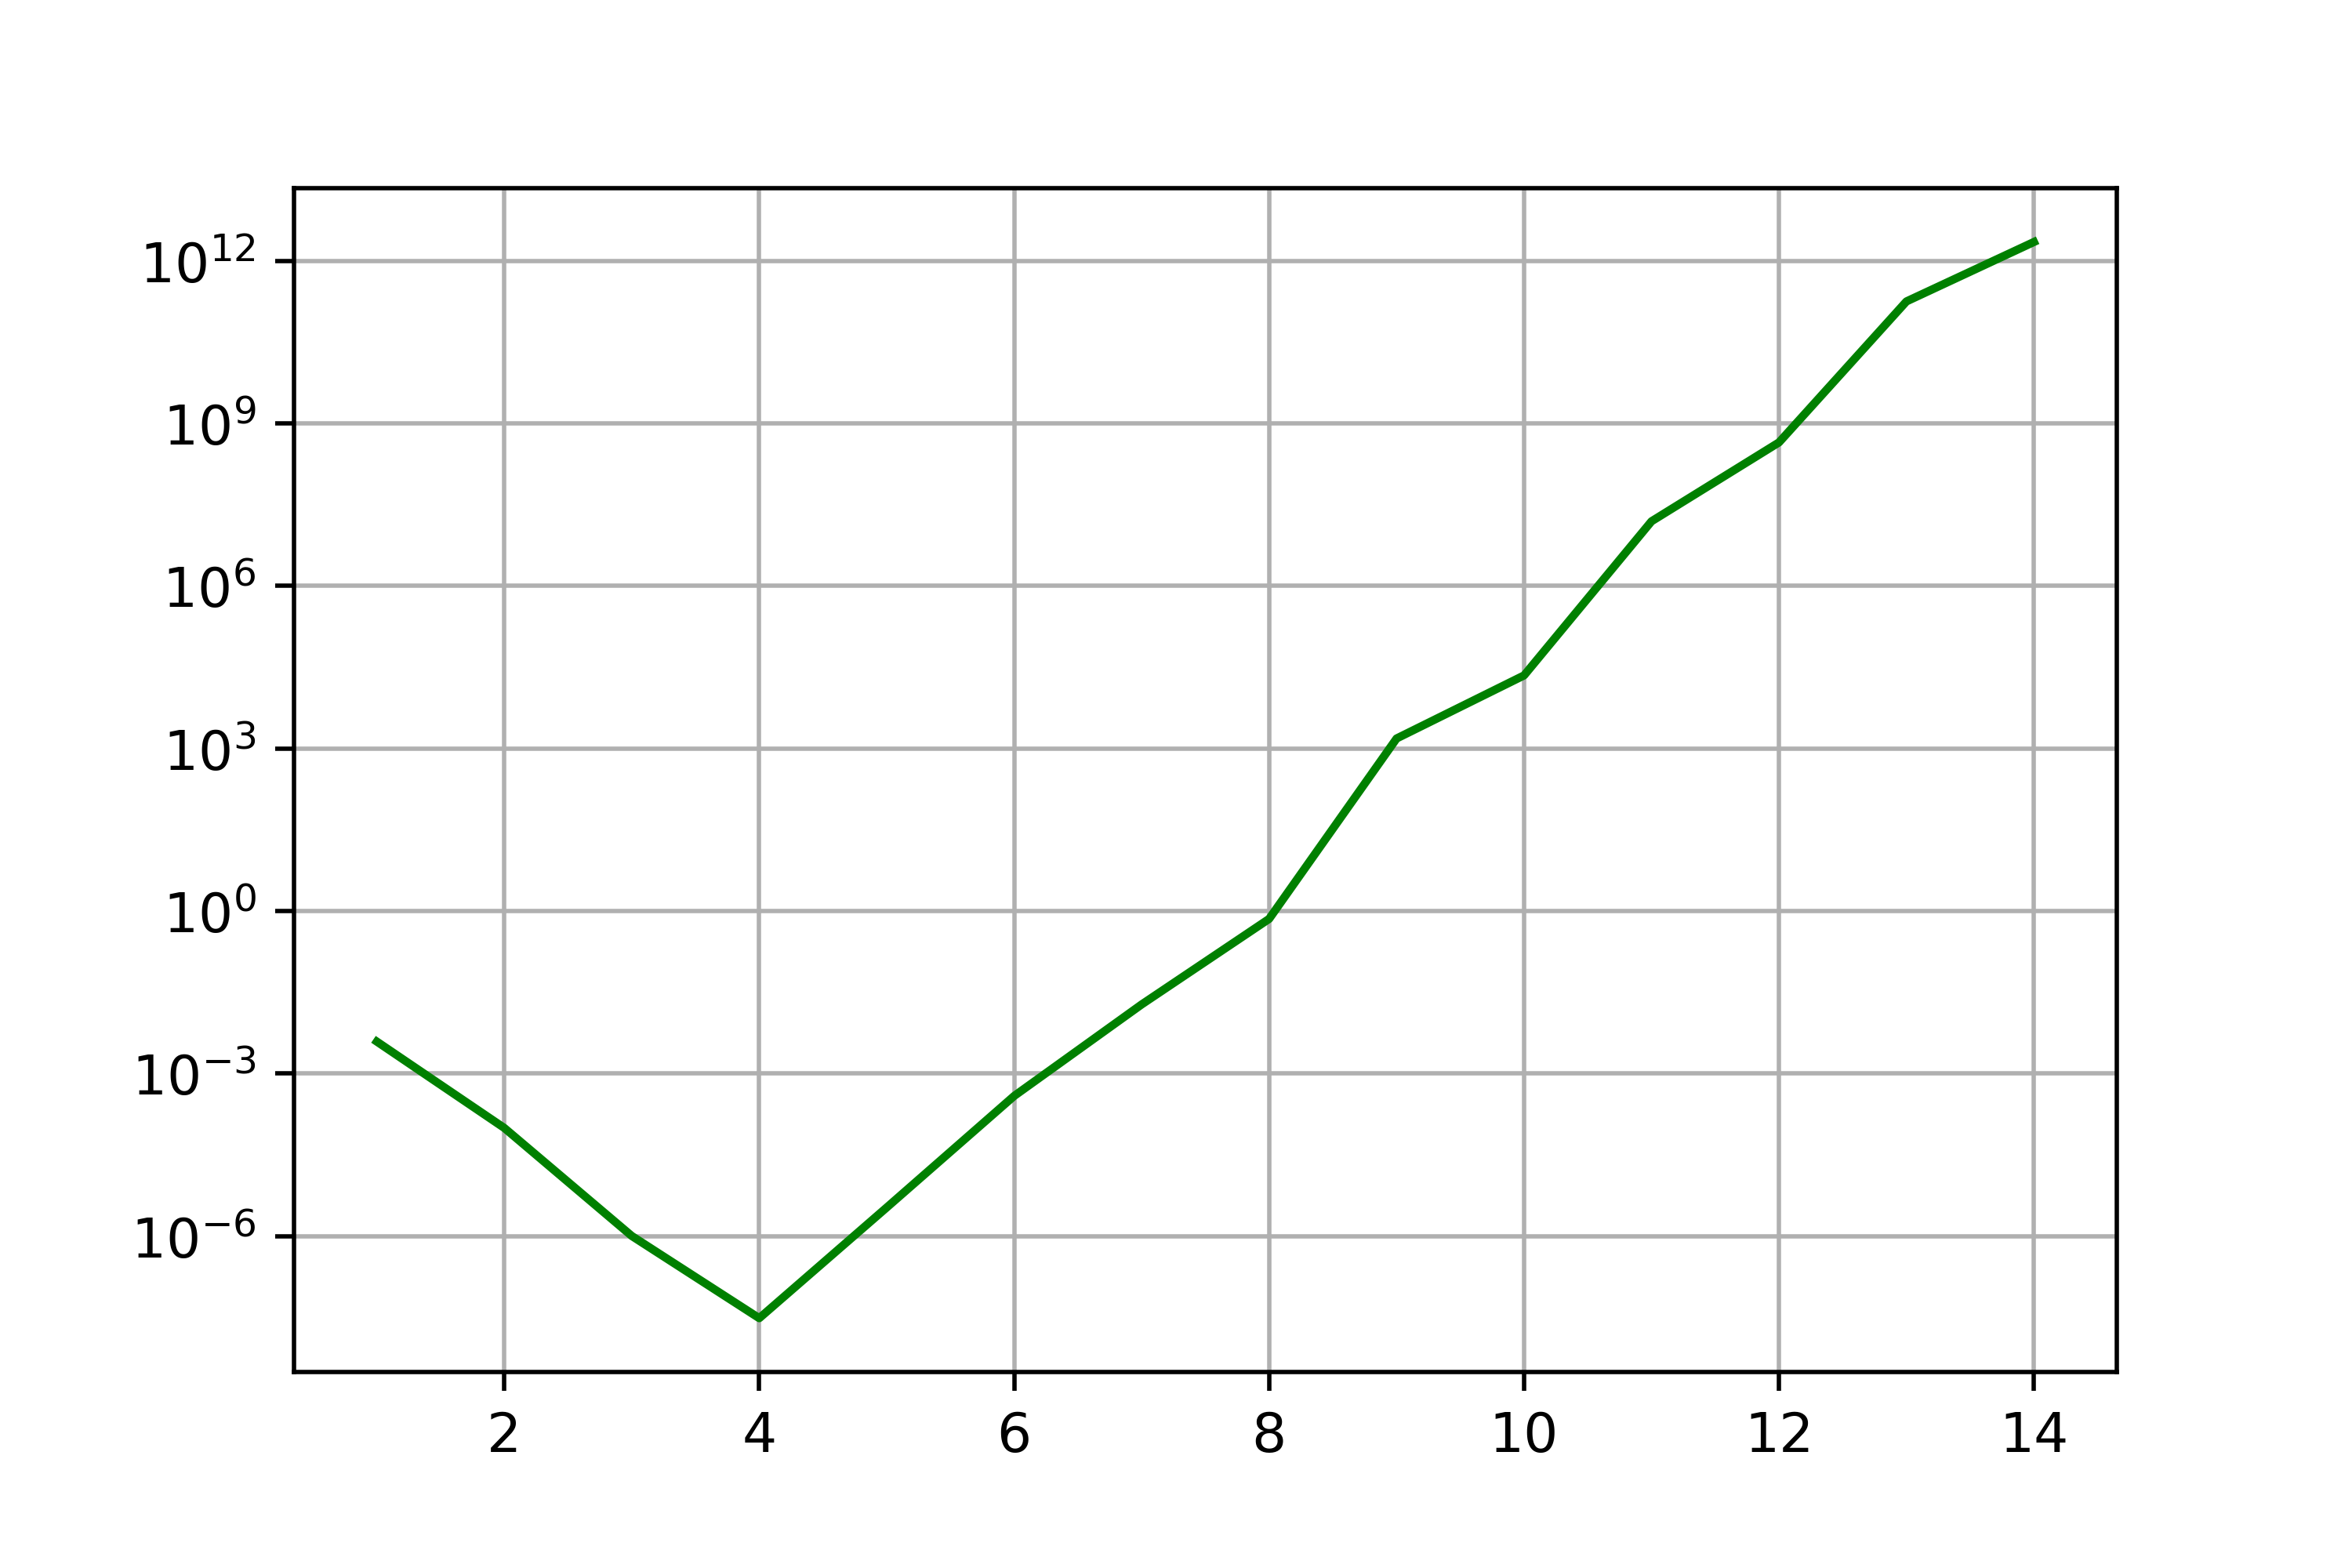
\includegraphics[width=8.5cm]{images/plot_6.1_2nd_deriv_err.png} % второе изображение
		\caption{Погрешность вычисления второй производной}
	\end{minipage}
\end{figure}

\[
\begin{tabular}{| p{3.75cm} | p{3.75cm} | p{3.75cm} | p{3.75cm} |}
	\hline
	$f'(c) = 13.83391227$ & Первый результат \newline при шаге $h = 10^{-1}$ & Наилучший результат \newline при шаге $h = 10^{-8}$ &  Последний результат \newline при шаге $h = 10^{-15}$ \\ \hline
	Формула (1) & $dl_1 = 14.33853900$ \newline $\Delta l_1 = 0.50462672$ &  $dl_1 = 13.83391252$ \newline $\Delta l_1 = 0.00000025$ &  $dl_{15} = 13.76676550$ \newline $\Delta l_{15} = 0.06714676$ \\ \hline
	Формула (2) & $dl_1 = 11.30169535$ \newline $\Delta l_1 = 2.53221691$ & $dl_1 = 13.83391221$ \newline $\Delta l_1 = 0.00000006$ &  $dl_{15} = 13.76676550$ \newline $\Delta l_{15} = 0.06714676$ \\ \hline
	$f''(c) = 30.37231240$ & Первый результат \newline при шаге $h = 10^{-1}$ & Наилучший результат \newline при шаге $h = 10^{-4}$ &  Последний результат \newline при шаге $h = 10^{-15}$ \\ \hline
	Формула (6) & $dl_1 = 30.36843645$ \newline $\Delta l_1 = 0.00387594$ &  $dl_1 = 30.37231237$ \newline $\Delta l_1 = 0.00000003$ &  $dl_{15} = 0.0$ \newline $\Delta l_{15} =30.37231240$ \\ \hline
\end{tabular}
\]

Выведем формулу (6) вычисления второй производной: $f''(x) \approx \dfrac{f(x + h) - 2f(x) + f(x - h)}{h^2}$
Для этого возьмем 3 узла интерполяции и построим по ним многочлен Ньютона 2 степени, а затем дважды продифференцируем его:

\begin{gather*}
	P_2(x) = f_i + \dfrac{\Delta f_i}{h}(x - x_i) + \dfrac{\Delta^2f_i}{2h^2}(x - x_i)(x - x_{i+1}) \\
	P_2'(x) =  \dfrac{\Delta f_i}{h} + \dfrac{\Delta^2f_i}{2h^2}((x - x_i) + (x - x_{i+1})) \\
	P_2''(x) = 2\dfrac{\Delta^2f_i}{2h^2} = \dfrac{f_{i+1} - 2f_i + f_{i-1}}{h^2}
\end{gather*}
\section*{Задача 6.2}
\subsection*{Постановка задачи}
Найти приближенное решение задачи Коши для обыкновенного дифференциального уравнения (ОДУ) 1-го порядка с точностью $\varepsilon = 10^{-6}$ на отрезке $[\pi/2, \pi/2 + 0.8]$.
\[
	\begin{cases}
		y' = -\dfrac{y}{t} + \dfrac{\cos{t}}{t} \\
		y(\pi/2) = 0
	\end{cases}
\]
\subsection*{Решение}
Найдем аналитическое решение:
\begin{gather*}
	y' + \dfrac{y}{t} = 0 \\
	y_{одн} = \dfrac{C(t)}{t}\\
	y_{одн}' = \dfrac{tC'(t) - C(t)}{t^2}\\
	y_{одн}' + \dfrac{y_{одн}}{t} = \dfrac{C'(t)}{t} - \dfrac{C(t)}{t^2} + \dfrac{C(t)}{t^2} = \dfrac{\cos{t}}{t} \\
	C'(t) = \cos{t} \\
	y = \dfrac{\sin{t}}{t} + \dfrac{C}{t}\\
	y = \dfrac{\sin{t}}{t} - \dfrac{1}{t}
\end{gather*}

Запишем расчетную формулу для метода Эйлера: $y_{i+1} = y_i + hf(t_i, y_i)$ и правило Рунге для данного метода: $y^{h/2}_i - y(t_i) \approx y^{h/2}_i - y^{h}_i$. При поиске решения с точностью $\varepsilon = 10^{-6}$ с помощью данного метода потребовалось 131073 точки, то есть шаг, на котором точность достигается равен $h = 6.103515625 \times 10^{-6}$.

При поиске решения с помощью экстраполяционного метода Адамса 3-го порядка, так как нам известно точное решение, зададим значения в точках $y_1 = y(a + h), y_2 = y(a + 2h)$ так как метод является 3-х точечным. Ниже представлена  расчетная формула данного метода. Для нахождения решения с заданной точностью потребовалось 65 точек, то есть величина шага составила $h = 0.0125$.
\[
	y_{i+1} = y_i + \dfrac{h}{12}[23f(t_i, y_i) - 16f(t_{i-1}, y_{i-1}) + 5f(t_{i-2}, y_{i-2})]
\]

Ниже на графиках представлены графики точного и приближенного решений, а также графики погрешностей.

\begin{figure}[h!]
	\centering                                                                                            
	\begin{minipage}{0.45\textwidth}
	        \centering
	        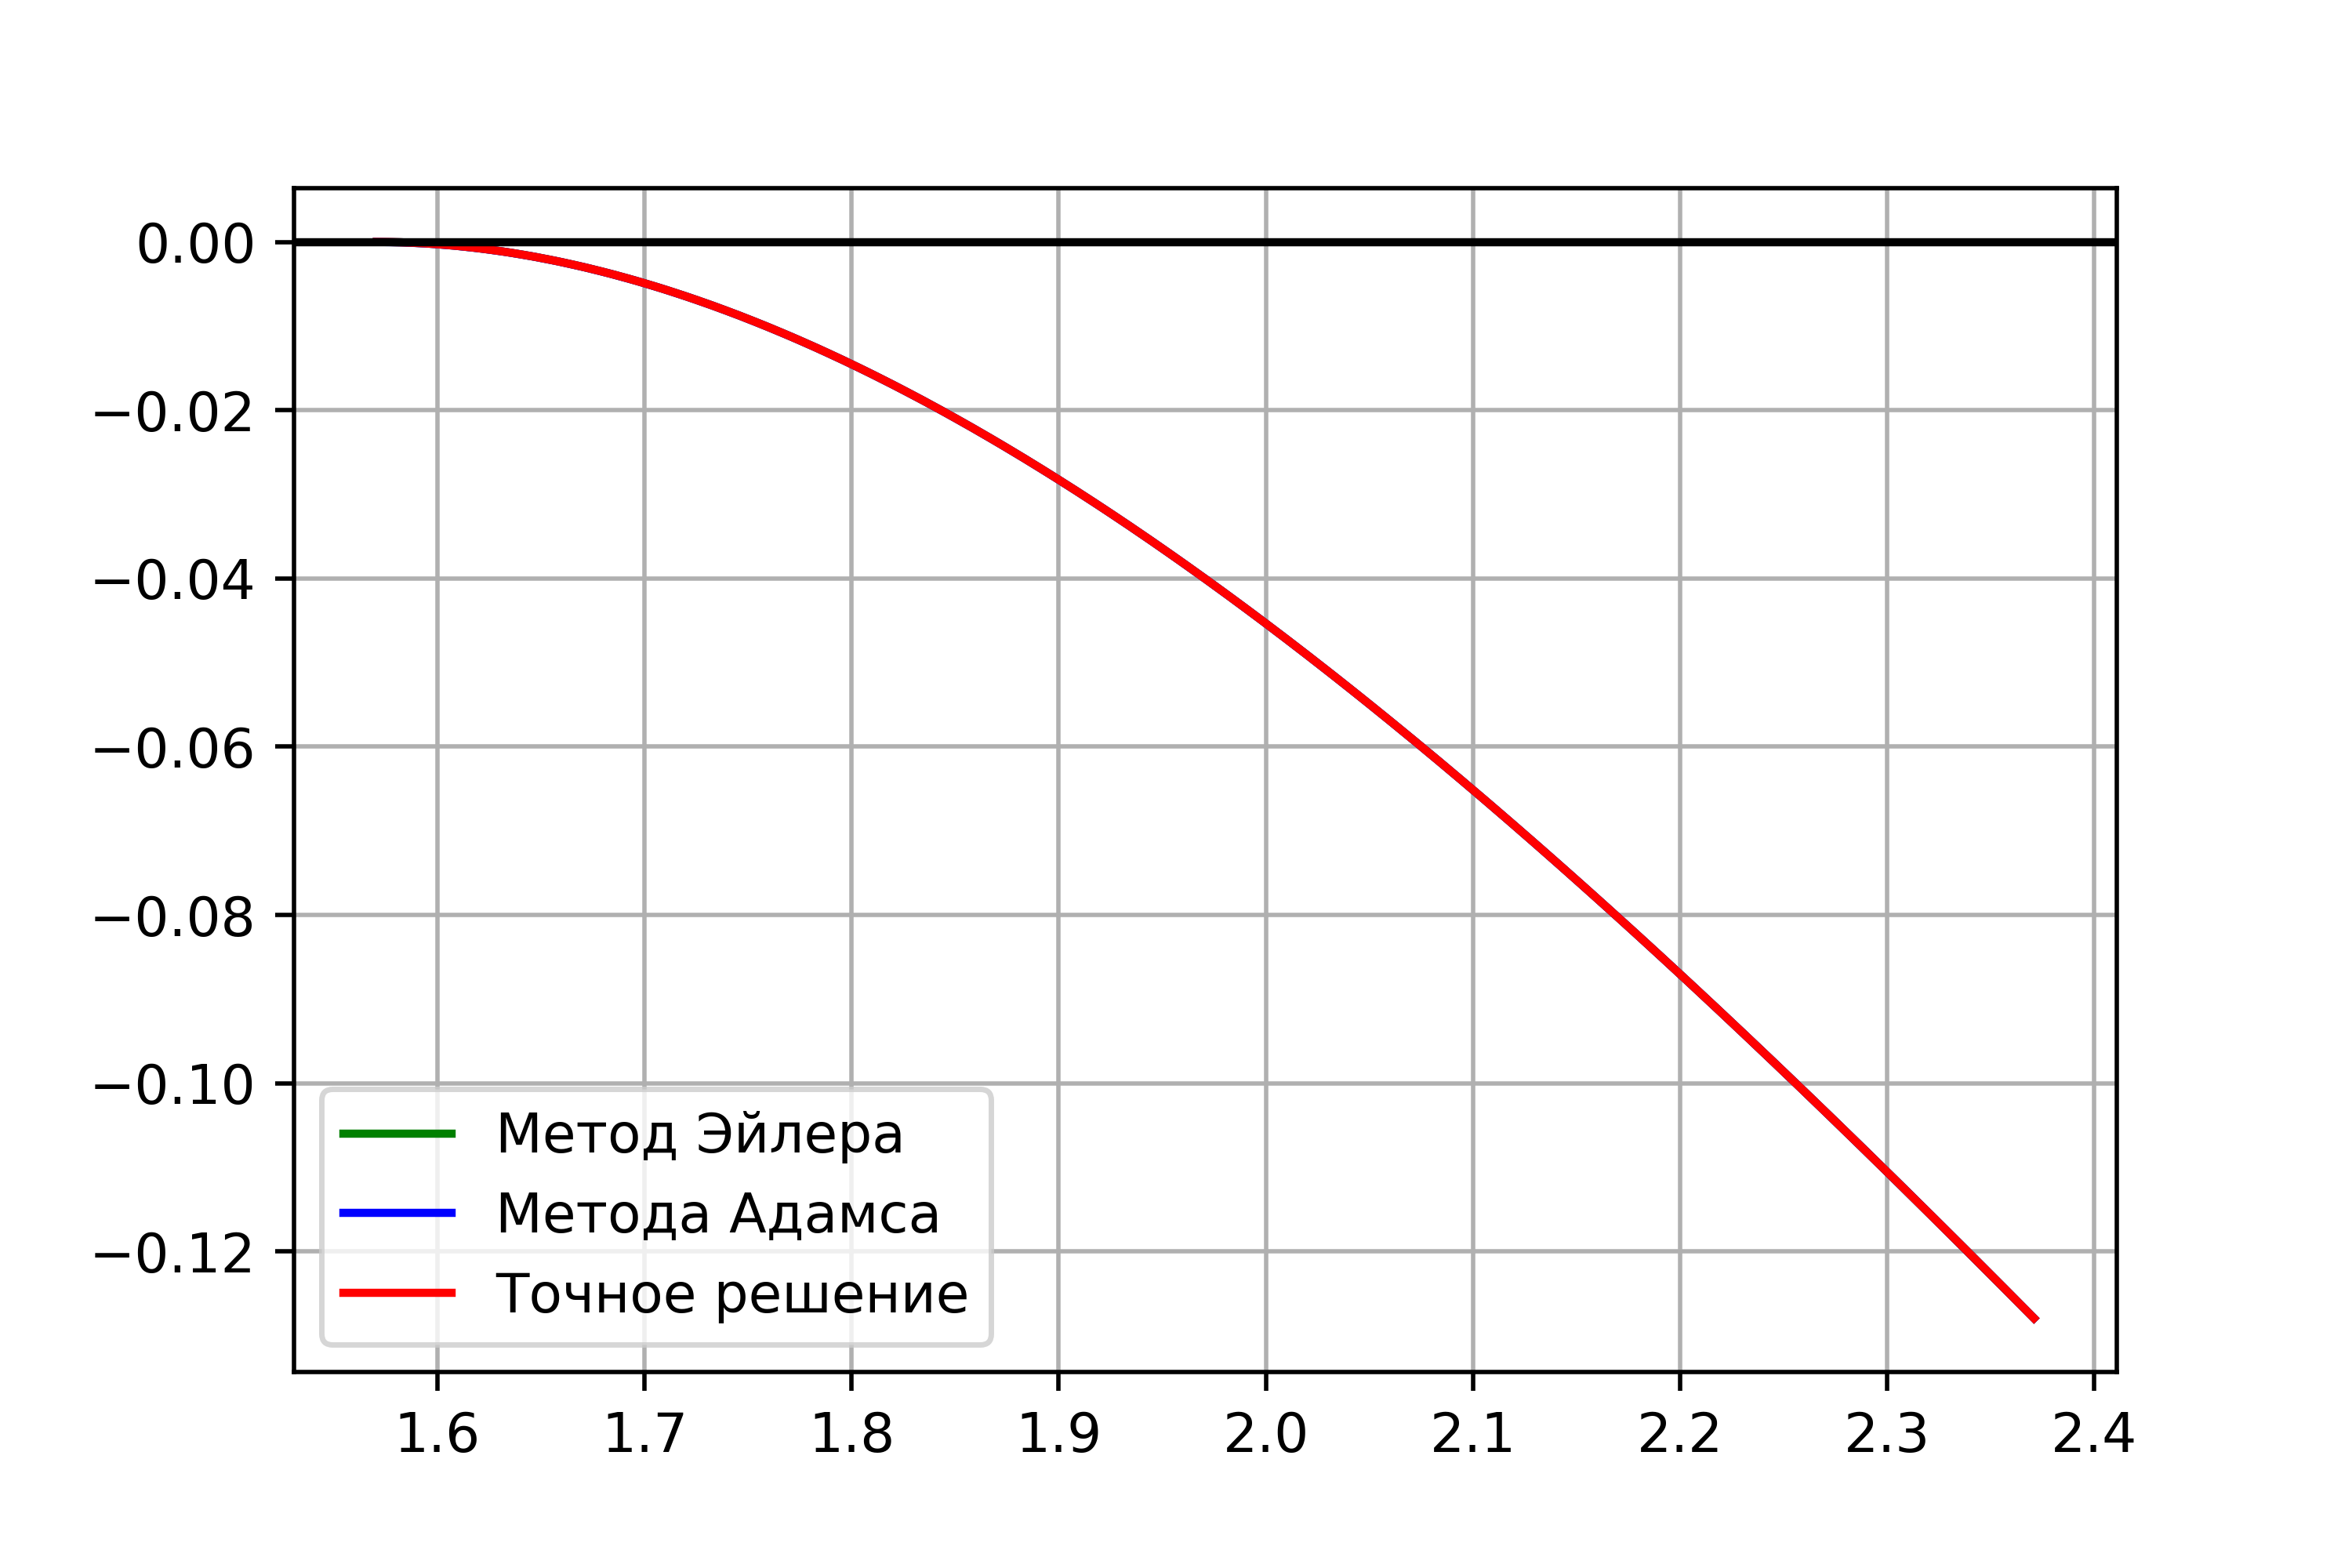
\includegraphics[width=8.5cm]{images/6.2_solution_plot.png} % первое изображение
	        \caption{Графики решений}
	\end{minipage}\hfill
	\begin{minipage}{0.45\textwidth}
		\centering
		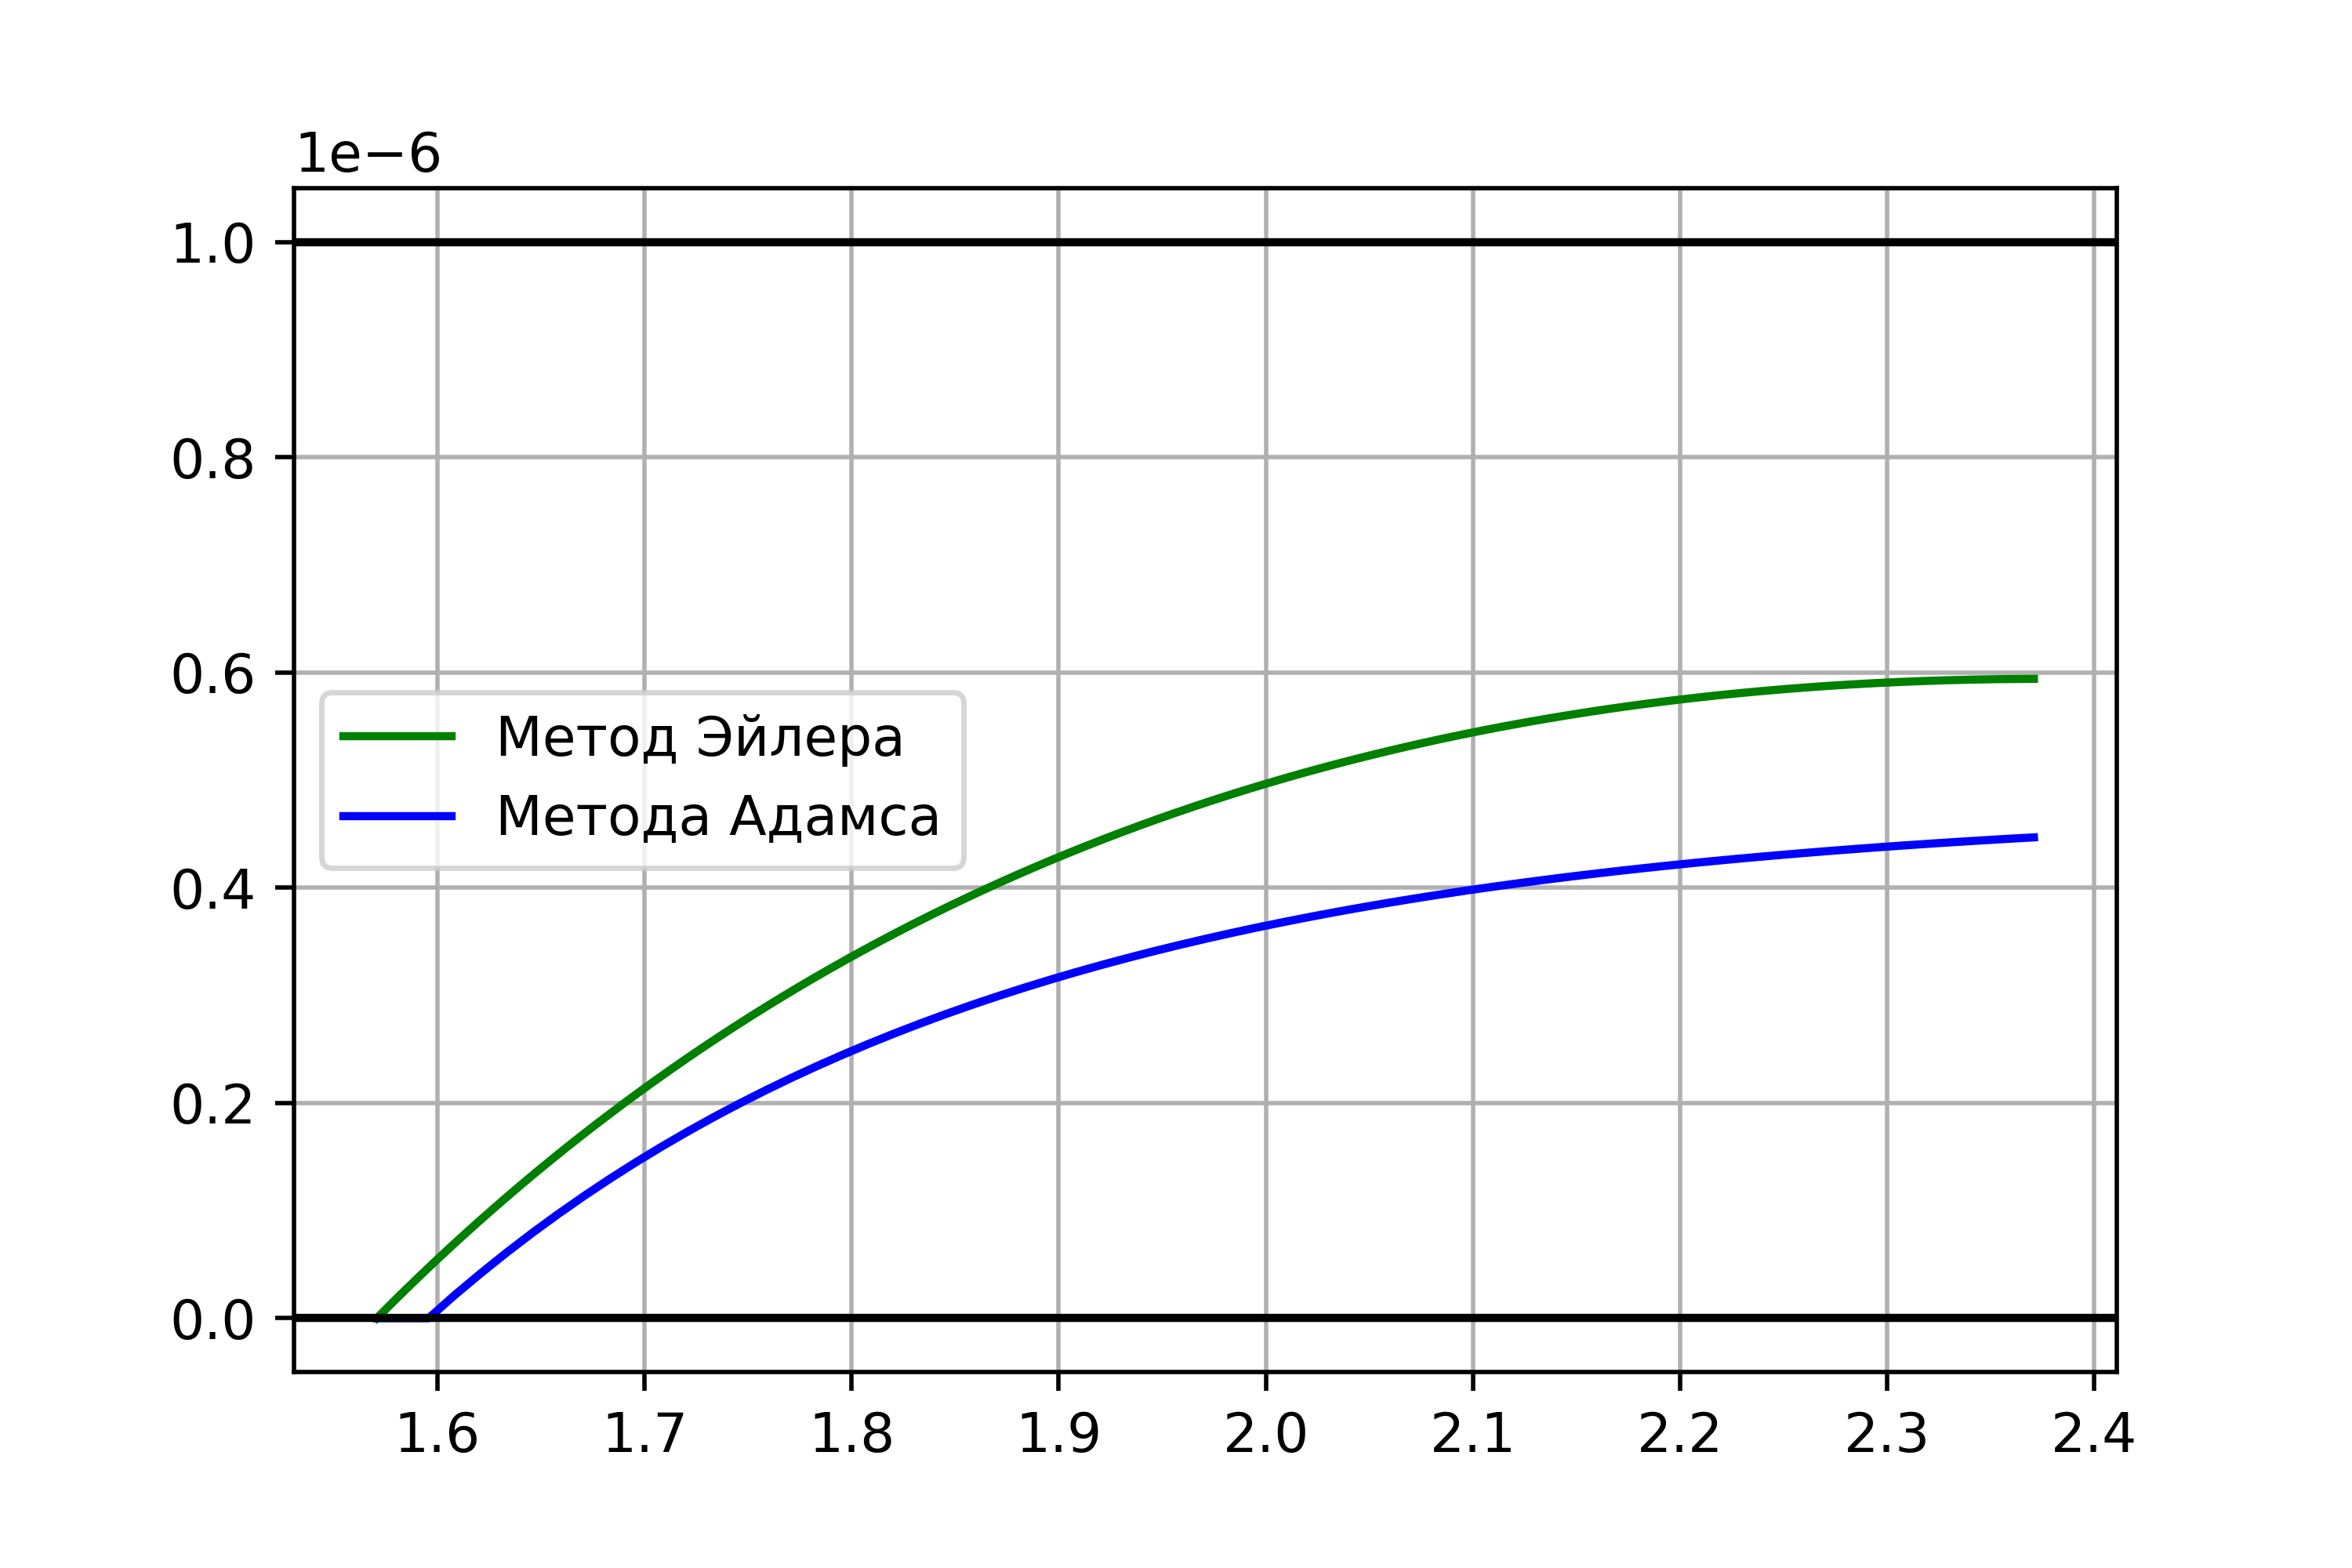
\includegraphics[width=8.5cm]{images/6.2_solution_err_plot.png} % второе изображение
		\caption{Погрешность нахождения решений}
	\end{minipage}
\end{figure}

На втором графике(Рис. 6) Видно, что метод Адамса показывает большую точность, причем на меньшем количестве узлов, что является результатом более высокого порядка точности данного метода по сравнению с методом Эйлера.

\end{document}